%
\documentclass[12pt,reqno]{amsart}
\usepackage{amssymb}
\usepackage{appendix}
\usepackage{tikz}
%\usepackage[showonlyrefs=true]{mathtools} %amsmath extension package
\usepackage{cancel}  %for cancelling terms explicity on pdf
\usepackage{yhmath}   %makes fourier transform look nicer, among other things
\usepackage{framed}  %for framing remarks, theorems, etc.
\usepackage{enumerate} %to change enumerate symbols
\usepackage[margin=2.5cm]{geometry}  %page layout
\setcounter{tocdepth}{1} %must come before secnumdepth--else, pain
\setcounter{secnumdepth}{1} %number only sections, not subsections
%\usepackage[pdftex]{graphicx} %for importing pictures into latex--pdf compilation
\numberwithin{equation}{section}  %eliminate need for keeping track of counters
%\numberwithin{figure}{section}
\setlength{\parindent}{0in} %no indentation of paragraphs after section title
\renewcommand{\baselinestretch}{1.1} %increases vert spacing of text
%
\usepackage{hyperref}
\hypersetup{colorlinks=true,
linkcolor=blue,
citecolor=blue,
urlcolor=blue,
}
\usepackage[alphabetic, initials, msc-links]{amsrefs} %for the bibliography; uses cite pkg. Must be loaded after hyperref, otherwise doesn't work properly (conflicts with cref in particular)
\usepackage{cleveref} %must be last loaded package to work properly
%
\newcommand{\ds}{\displaystyle}
\newcommand{\ts}{\textstyle}
\newcommand{\nin}{\noindent}
\newcommand{\rr}{\mathbb{R}}
\newcommand{\nn}{\mathbb{N}}
\newcommand{\zz}{\mathbb{Z}}
\newcommand{\cc}{\mathbb{C}}
\newcommand{\ci}{\mathbb{T}}
\newcommand{\zzdot}{\dot{\zz}}
\newcommand{\wh}{\widehat}
\newcommand{\p}{\partial}
\newcommand{\ee}{\varepsilon}
\newcommand{\vp}{\varphi}
\newcommand{\wt}{\widetilde}
%
%
%
%
\newtheorem{theorem}{Theorem}[section]
\newtheorem{lemma}[theorem]{Lemma}
\newtheorem{corollary}[theorem]{Corollary}
\newtheorem{claim}[theorem]{Claim}
\newtheorem{prop}[theorem]{Proposition}
\newtheorem{proposition}[theorem]{Proposition}
\newtheorem{no}[theorem]{Notation}
\newtheorem{definition}[theorem]{Definition}
\newtheorem{remark}[theorem]{Remark}
\newtheorem{examp}{Example}[section]
\newtheorem{exercise}[theorem]{Exercise}
%
%\makeatletter \renewenvironment{proof}[1][\proofname] {\par\pushQED{\qed}\normalfont\topsep6\p@\@plus6\p@\relax\trivlist\item[\hskip\labelsep\bfseries#1\@addpunct{.}]\ignorespaces}{\popQED\endtrivlist\@endpefalse} \makeatother%
%makes proof environment bold instead of italic
\newcommand{\uol}{u^\omega_\lambda}
\newcommand{\lbar}{\bar{l}}
\renewcommand{\l}{\lambda}
\newcommand{\R}{\mathbb{R}}
\newcommand{\RR}{\mathcal{R}}
\newcommand{\al}{\alpha}
\newcommand{\ve}{q}
\newcommand{\tg}{{tan}}
\newcommand{\m}{q}
\newcommand{\N}{N}
\newcommand{\ta}{{\tilde{a}}}
\newcommand{\tb}{{\tilde{b}}}
\newcommand{\tc}{{\tilde{c}}}
\newcommand{\tS}{{\tilde{S}}}
\newcommand{\tP}{{\tilde{P}}}
\newcommand{\tu}{{\tilde{u}}}
\newcommand{\tw}{{\tilde{w}}}
\newcommand{\tA}{{\tilde{A}}}
\newcommand{\tX}{{\tilde{X}}}
\newcommand{\tphi}{{\tilde{\phi}}}
\synctex=1
\begin{document}
\title{Strategy for Proof of Sharp $G^{2}$ Regularity in Time for NLS}
\author{Alex Himonas, David Karapetyan, and Gerson Petronilho}
\date{\today}
%
\maketitle
%
%
%
%
%
%
\section{Sharp $G^2$ regularity in time for NLS} 
\label{pg2-rreg-3}
%
%
Recall the cubic non-linear Schr\"odinger (NLS) Cauchy problem 
%
%
\begin{gather}
  \label{peqn:nls-t}
  \partial_{t}u + i\partial_{x}^2u+i |u|^2u,
  \\
  \label{peqn:nls-t-data}
  u(x,0)=\varphi(x) \in \mathcal{C}^\omega(\mathbb{T}).
\end{gather}
%
We would like to
prove the following.
%
%
%%%%%%%%%%%%%%%%%%%%%%%%%%%%%%%%%%%%%%%%%%%%%%%%%%%%%
%
%
%                
%
%
%%%%%%%%%%%%%%%%%%%%%%%%%%%%%%%%%%%%%%%%%%%%%%%%%%%%%
%
%
\begin{theorem}
  Solutions to the Cauchy problem \eqref{peqn:nls-t}-\eqref{peqn:nls-t-data}
  are not in general better than $G^{2}$ in time. More precisely, there exists
  $\vp \in  \mathcal{C}^\omega(\mathbb{T})$ such that the associated solution
  $u(x,t)$ to \eqref{peqn:nls-t} is not $G^{\sigma}$ in time for any $1 \le \sigma <
  2$. 
\label{thm:sharp}
\end{theorem}
%
%
I don't know how to prove this yet. Instead, I am interested in proving a slightly
weaker result, using the $G^{\sigma, \delta}$ spaces,
which we define to be the completion
of $L^{2}(\ci^{2})$ under the norm
%
%
\begin{equation*}
  \begin{split}
    \| u \|^{2}_{G^{\sigma, \delta}} = \sum_{n, \tau \in \zz} \langle
    \tau - n^{2} \rangle  [(\min \{ |\tau -1 |, |\tau + 1| \})!]^{2 \sigma}
    e^{2 \delta n} | \wh{u}(n, \tau) |^{2} 
  \end{split}
\end{equation*}
%
where we adopt the notation
%
%
\begin{equation*}
  \begin{split}
    \langle k \rangle  = 1 + | k |, \quad k \in \rr.
  \end{split}
\end{equation*}
%
\begin{framed}
  I have not seen the spaces $G^{\sigma, \delta}$ anywhere in the
  literature. However, they seem reasonable, as they are a natural extension of
  the Foias-Temam spaces used in your earlier work with Alex.
\end{framed}
%
%
The slightly weaker result I want to prove
is as follows.
%
\begin{theorem}
  Fix $\delta > 0$. Then exists
  $\vp \in  \mathcal{C}^\omega(\mathbb{T})$ such that the associated solution
  $u(x,t)$ to \eqref{peqn:nls-t} is not in $G^{\sigma, \delta}$
  in time for any $1 \le \sigma < 2$. 
\label{thm:sharp-weak}
\end{theorem}
%
Recall the Bourgain space $X \doteq X^{0,1/2}$ adapted to the problem of proving
$L^{2}$ well-posedness of
NLS, with norm given by
%
\begin{equation*}
  \begin{split}
    \| u \|_{X}^{2} = \sum_{n, \tau \in \zz} \langle \tau - n^{2} \rangle 
    | \wh{u}(n, \tau) |^{2}.
  \end{split}
\end{equation*}
%
%
What is important to observe is that $G^{\sigma, \delta} \subset X$
continuously. Furthermore, we have the following important property. %
%
%
%
%
%
%%%%%%%%%%%%%%%%%%%%%%%%%%%%%%%%%%%%%%%%%%%%%%%%%%%%%
%
%
\begin{lemma}
  Fix $\sigma \ge 1$ and $\delta > 0$.
  If $u \in G^{\sigma, \delta}$, then $u \in G^{\sigma}(\ci,
  \mathcal{C}^{\omega})$.
\label{lem:main-space-embed}
\end{lemma}
%
%
%
\begin{proof}
  If $u \in G^{\sigma, \delta}$, then we must have
  %
  %
  \begin{equation*}
    \begin{split}
      | \wh{u}(n, \tau) |
      & <  \langle \tau - n^{2} \rangle^{1/2}    e^{-\delta n}
      [(\min \{|\tau -1 |, |\tau + 1|\})!]^{\sigma}
      \\
      & <  \langle \tau - n^{2} \rangle e^{-\delta n}
      [(\min \{ |\tau -1 |, |\tau + 1| \})!]^{\sigma}
      \\
      & \lesssim \langle \tau \rangle \langle n \rangle ^{2}
      e^{-\delta n}
      [(\min \{ |\tau -1 |, |\tau + 1| \})!]^{sigma}
      \\
      & < \langle n \rangle ^{2}
      e^{-\delta n}
      (| \tau |)!^{\sigma}
      \\
      & < C_{\delta} e^{-\delta n/2} (| \tau |)!^{\sigma}
    \end{split}
  \end{equation*}
  %
  which completes the proof. 
  %
\end{proof}
%
%
%
\begin{proof}[Proof of Theorem~\ref{thm:sharp-weak}]
  %
  %
  We rewrite the NLS Cauchy problem as a time localized integral equation   
  %
  \begin{equation*}
    \begin{split}
      u(x,t)
      & = \psi(t) e^{it \Delta} \vp + \psi(t)
      \int_{0}^{t} e^{i(t - t') \Delta}(u u \bar{u})
      dt'
      \\
      & = T(u)
    \end{split}
  \end{equation*}
  %
  %
  where $\psi$ is a smooth
  cutoff function symmetric about the origin, and $T = T_{\vp}$. Since we have
  introduced a cutoff in time, we may without loss of generality
  (via periodic extension) view the time
  variable as being periodic, with the length of the period equal to the support
  of $\psi$. From the well-posedness theory of NLS, for sufficiently small initial
  data $\vp \in L^{2}(\ci)$, $T$ is a contraction on
  $B_{X}(R)$ (the ball in $X$ centered at zero of radius $R$), where $R =
  R(\|\vp \|_{L^{2}})$. Proceeding by contradiction, assume that the picard
  iteration starting at a point in $B_{X}(R)$ converges (in $X$)
  to a solution $u(x,t) \in G^{\sigma, \delta}$.
  Then from the continuous embedding $G^{\sigma, \delta} \subset X$ it follows
  that $T_{\vp}$ is a contraction on $B_{G^{\sigma, \delta}}(R)$. 
  \\
  \\
  \begin{center}
    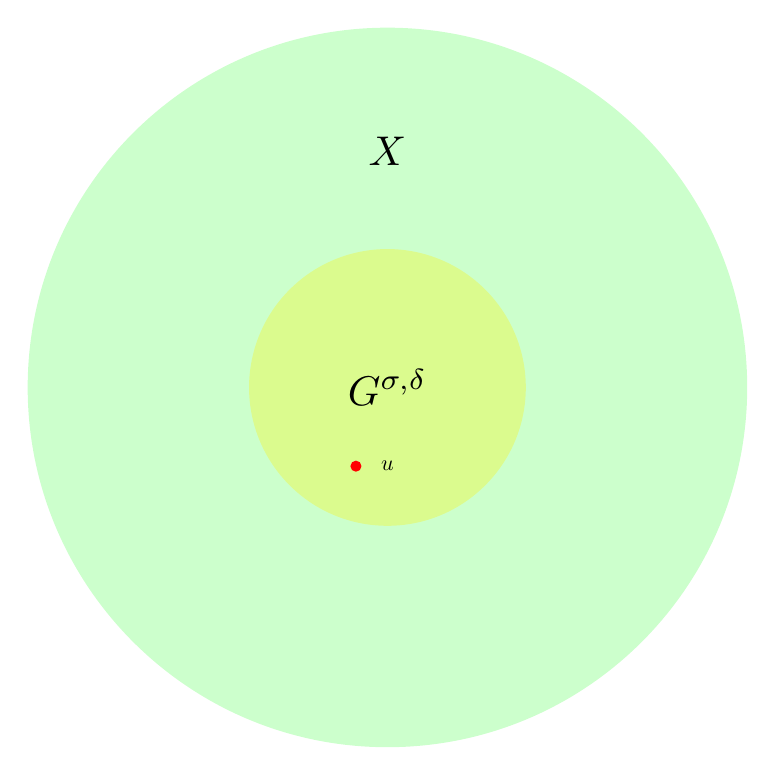
\begin{tikzpicture}
      \fill[color=green, opacity=0.2] (0,0) circle  (130pt);
      \fill[color=yellow, opacity=0.3] (0,0) circle  (50pt); 
      \fill[color=red] (-0.4,-1) circle  (2pt); 
      \draw (0, 3) node[scale=1.5] {$X$};
      \draw (0,0) node[scale=1.5] {$G^{\sigma, \delta}$};
      \draw (0,-1) node[scale=0.8] {$u$};
    \end{tikzpicture}
  \end{center}
  But this is
  impossible, due to the following key proposition.
  %
  %
  %%%%%%%%%%%%%%%%%%%%%%%%%%%%%%%%%%%%%%%%%%%%%%%%%%%%%
  %
  %
  %                non-contraction
  %
  %
  %%%%%%%%%%%%%%%%%%%%%%%%%%%%%%%%%%%%%%%%%%%%%%%%%%%%%
  %
  %
  \begin{proposition}[Key Result We'd Like to Prove]
      Fix $\delta > 0$, $1 < \sigma < 2$. Then there exists
      $\vp \in \mathcal{C}^{\omega}$ such that for
      any $u \in G^{\sigma, \delta}$, we have
      \begin{equation}
          \| T_{\vp}(u) \|_{G^{\sigma, \delta}} > \|u \|_{G^{\sigma, \delta}}.
      \end{equation}
      \label{prop:non-cont}
  \end{proposition}
  %
  %
  By contradiction, the proof is complete. 
\end{proof}

\section{Another Strategy} 
\label{sec:another-strat}
Substituting the ansatz $u = f + ig$, where $f = f(x), g(x)$ are real valued into the NLS ivp, we get
%
%
\begin{equation*}
\begin{split}
  i \p_{t}(f + ig) + \p_{x}^{2}(f + ig) + | f + ig |^{2}(f + ig) = 0
\end{split}
\end{equation*}
%
%
or
%
%
\begin{equation*}
\begin{split}
  if_{t} - g_{t} + f_{xx} + ig_{xx} + f^{3} + if^{2}g + fg^{2} + ig^{3}=0.
\end{split}
\end{equation*}
%
%
Then we must have
\begin{gather*}
  if_{t} + ig_{xx} + if^{2}g + ig^{3}=0,
  \\
  -g_{t} + f_{xx} + f^{3} + fg^{2} = 0.
\end{gather*}
Hence, solving the NLS ivp is equivalent to solving the system

\begin{gather}
  if_{t} = -ig_{xx} - if^{2}g - ig^{3},
  \label{hj}
  \\
  g_{t} = f_{xx} + f^{3} + fg^{2},
  \label{hh}
  \\
  f(x,0) = f_{0}(x),
  \\
  g(x,0) = g_{0}(x).
\end{gather}

Now, if $g_{0}(x) = 0$, then from \eqref{hj} we see that $f_{t}(0) = 0$, and so itis impossible to get failure of analyticity in time at $0$ in this case. But notice, all the terms on the right hand side of \eqref{hj} are negative, and all terms on the right hand side of \eqref{hh} are positive. Hence, we can apply the Himonas-Petronilho machinery.
\end{document}
%\nocite{*}
\bibliography{/Users/davidkarapetyan/math/bib-files/references.bib}
